\documentclass[../ana1.tex]{subfiles}
\onlyinsubfile{\sectionNumbering} %Use numbering relative to sections and not subsection

\begin{document}
\setcounter{section}{18}
\section{Satz von Rolle, Mittelwertsatz, Extrema}
\begin{defi}[Lokale Extrema]
    Die Funktion \( f : [a,b] \rightarrow \R \) (oder \( (a,b) \))
    hat in \( x_0 \in [a,b] \) ein lokales Minimum (oder in 
    \( x_0 \in (a,b) \)), falls \( \exists \, \delta > 0 \), 
    sodass 
    \[ f(x_0) \leq f(x) \, \forall \, x \in U_\delta(x_0)
    \cap [a,b] = (x_0 - \delta, x_0 + \delta) \cap [a,b] \]
    Ist \( x_0 \in (a,b) \), so kann \( \delta > 0 \) so klein 
    gewählt werden, dass \( (x_0 - \delta, x_0 + \delta) 
    \cap [a,b] = (x_0 - \delta, x_0 + \delta) \).
    \begin{center}
    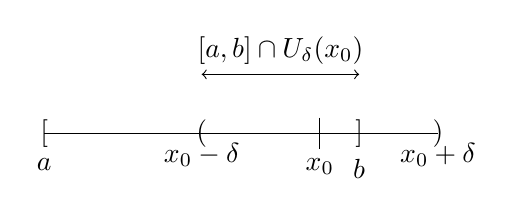
\begin{tikzpicture}
        \draw (0,0) -- (5,0);
        \draw (0,0) node {\([\)} node[below=2mm] {\(a\)};
        \draw (4,0) node {\(]\)} node[below=2mm] {\(b\)};
        \draw (3.5,0.2) -- (3.5,-0.2) node[below] {\(x_0\)};
        \draw (2,0) node {\((\)} node[below] {\( x_0 - \delta \)};
        \draw (5,0) node {\()\)} node[below] {\( x_0 + \delta \)};
        \draw[<->] (2,0.75) -- (4,0.75) node[midway,above] {\( [a,b] \cap U_\delta(x_0) \)};
    \end{tikzpicture}
    \end{center}
    Ist sogar \( f(x_0) < f(x) \,\forall \, x \in 
    (x_0 - \delta, x_0 + \delta) \cap [a,b] \), so heißt 
    das lokale Minimum isoliert (oder strikt).\\
    Analog: \( f \) hat in \( x_0 \) ein (indirektes) lokales 
    Maximum, falls \(-f\) in \(x_0\) ein (isoliertes) lokales 
    Minimum hat.\\
    Lokale Extrema \(=\) lokale Minima oder Maxima.
\end{defi}
\begin{satz}
    \( f: (a,b) \rightarrow \R \) habe in \(x_0 \in (a,b) \) 
    ein lokales Extremum. Ist \(f\) in \(x_0\) differenzierbar, 
    so gilt \( f'(x_0) = 0 \) (notwendige Bedingung für Extrema).
\end{satz}
\begin{bew}
    O.\ B.\ d.\ A.\ sei \(x_0\) ein lokales Minimum von \(f\) 
    (sonst betrachte \(-f\)).
    \[ \Rightarrow \exists \, \delta > 0 : f(x) \geq f(x_0) 
    \,\forall x \in (x_0 - \delta, x_0 + \delta) \]
    \[ \Rightarrow \frac{f(x) - f(x_0)}{x - x_0} = \begin{cases}
        \geq 0, &x \in (x_0, x_0 + \delta)\\
        \leq 0, &x \in (x_0 - \delta, x_0)
    \end{cases} \]
    \[ \Rightarrow f_+'(x_0) = \limesx{x}{x_0 +} 
    \frac{ f(x) - f(x_0) }{ x - x_0 } \geq 0 \]
    \[ = f_{\minus}'(x_0) = \limesx{x}{x_0 \minus} 
    \frac{ f(x) - f(x_0) }{ x - x_0 } \leq 0 \]
    \[ \Rightarrow f'(x_0) = f_{\pm}'(x_0) = 0. \]
    Rand: \(f: [a,b] \rightarrow \R \) \\
    hat lokales Minimum bei \( x_0 = b \).
    \[ \Rightarrow \frac{ f(x) - f(b) }{ x - b } \leq 0 \]
    \[ \Rightarrow f_{\minus}'(b) \leq 0. \]
\end{bew}
\begin{satz}[Rolle]
    Sei \( f: [a,b] \rightarrow \R \) stetig und differenzierbar 
    in \( (a,b) \) mit \( f(a) = f(b) = 0 \).
    \[ \Rightarrow \exists \, \xi \in (a,b) : f'(\xi) = 0. \]
\end{satz}
\begin{bew}
    \( [a,b]\) ist kompakt und \(f\) ist stetig.
    \[ \Rightarrow \exists \, \xi_1 \in [a,b], \xi_2 \in [a,b]: \]
    \[ f(\xi_1) = \sup( f(x), x \in [a,b] ), f(\xi_2) 
    = \inf (f(x) : x \in [a,b]). \]
    \( \Rightarrow \) Ist \( \xi_1 \in (a,b) \), nehme 
    \( \xi := \xi_1 \overset{\text{Satz 2}}{\Rightarrow}
     f'(\xi) = 0 \).\\
    Ist \( \xi_2 \in (a,b) \), nehme \( \xi := \xi_2 \)
    \( \oversett{Satz 2}{\Rightarrow} f'(\xi) = 0 \).\\
    Sind \( \xi_1, \xi_2 \in [a,b] \)
    \[ \sup(f(x) : x\in [a,b]) = \inf(\ldots) = 0. \]
    Also ist \( f(x) = 0 \,\forall \, x\in [a,b] \)
    \[ \Rightarrow f'(x) = 0 \, \forall \, x\in (a,b). \]
\end{bew}
\begin{satz}[Mittelwertsatz]
    \( f: [a, b] \rightarrow \R \) stetig und differenzierbar 
    auf \((a,b)\) 
    \[ \exists \, \xi \in (a,b): f'(\xi) = \frac{f(b)-f(a)}{b-a} \]
\end{satz}
\begin{bew}
    \( h(x) :=  f(x) - \left[f(a) + \frac{f(b)-f(a)}{b-a} 
    \cdot (x-a) \right] \) \\
    \( \Rightarrow h: [a,b] \rightarrow \R \) stetig und 
    differenzierbar auf \( (a,b) \) und 
    \[ h(a) = 0 = h(b) \oversett{Rolle}{\Rightarrow} 
    \exists \, \xi \in (a,b): 0 = h'(\xi) = f'(\xi) 
    - \frac{f(b)-f(a)}{b-a} \]
    \[ \Rightarrow f'(\xi) = \frac{f(b)-f(a)}{b-a}. \]
\end{bew}
\end{document}